\section{Neural Network}
Neural Network terinspirasi dari cara kerja neuron yang ada pada otak manusia, neuron bertugas sebagai penerima stimulus/rangsangan dan pengirim informasi yang akan diolah atau diproses oleh otak menjadi suatu output. Neuron merupakan sistem saraf pusat dan terdapat sekitar 100 miliar neuron yang ada pada tubuh manusia. Perhatikan gambar \ref{neuron}
\begin{figure}[H]
        \centerline{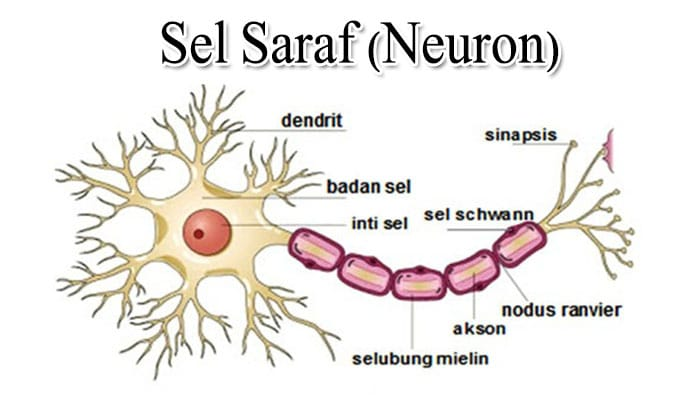
\includegraphics[scale=.45]{figures/neuron}}
        \caption{Sel Saraf (Neuron)}
		\label{neuron}
\end{figure}

Neuron terdiri dari 3 bagian yaitu akson (akar), soma (batang), dan dendrite (cabang). Neuron juga dibedakan menjadi 3 yaitu neuron sensorik atau sel saraf indra karena fungsinya yang berhubungan dengan penerima (indra) dan saraf pusat (otak dan sumsum tulang belakang). Neuron motorik atau sel saraf penggerak yang berfungsi membawa rangsangan dari saraf pusat (otak dan sumsum tulang belakang) ke otot. Terakhir yaitu neuron asosiasi ataus sel saraf penghubung, sel ini menghubungkan atau meneruskan rangsangan dari sel saraf sensorik ke sel saraf motorik.

Tiap neuron yang ada dalam otak kita saling terhubung dan berkirim informasi atau rangsangan berupa neurotransmitter, neuron yang saling berinteraksi dengan mengirimkan rangsangan ini akan menghasilkan kemampuan tertentu pada kerja otak kita. Contohnya, ketika kita bertemu dengan seorang kenalan yang menyapa kita maka otak akan berkerja sehingga dapat mengenali orang tersebut dan akan menghasilkan respon atau output, outputnya bisa berupa sapaan, lambaian tangan, obrolan, dan hal-hal lainnya yang biasa kita lakukan apabila bertemu dengan seseorang yang kita kenal. Jadi secara ilmiahnya, inputan atau rangsangan yang diterima yaitu berupa sapaan dari orang yang dikenali. Rangsangan ini akan diterima oleh alat indra (mata, telinga, hidung, lidah, dan kulit) melalui sel reseptor, kemudian akan diteruskan dalam bentuk impuls berupa arus listrik yang diteruskan ke sel saraf sensorik melalui sinapsis, lalu melewati sel saraf konektor menuju otak. Pada otak informasi akan diolah terlebi dahulu kemudian dikirimkan ke sel saraf motorik dan memberikan atau menghasilkan reaksi berupa sapaan, gerakan berupa lambaian tangan dll. Inilah proses kerja otak manusia begitupun dengan neural network yang terinspirasi dari cara neuron bekerja pada otak manusia. Siapa sangka mesin yang merupakan benda mati akan bisa berprilaku dan berkerja seperti layaknya manusia. Hingga saat ini sangat banyak diminati dan terus dikembangkan dengan tujuan dapat membantu memudahkan manusia dalam bekerja.

\subsection{Sejarah Neural Network}
\begin{figure}[H]
        \centerline{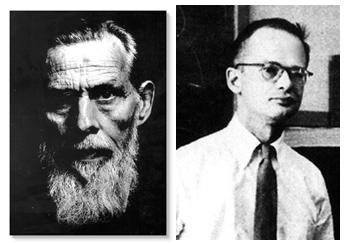
\includegraphics[scale=1]{figures/nn1}}
        \caption{McCulloch dan Pitts, penemu pertama Neural Network}
		\label{penemu}
\end{figure}
Neural Network bermula ketika Warren McMulloch yang merupakan seorang neurofisiologi dan Walter Pitts yang merupakan seorang ahli matematika menulis makalah tentang cara kerja dari neuron pada tahun 1943. Kemudian diperkuatnya konsep neuron dalam buku yang ditulis oleh Donald Hebb pada tahun 1949 yang berjudul The Organization of Behavior yang menunjukkan bahwa jaringan syaraf akan bertambah kuat setiap kali digunakan. Kemudian dilanjutkan dengan penelitian di IBM untuk mensimulasikan neural network tahun 1950 yang dipimpin oleh Nathanial Rochester.

Dengan diadakannya konferensi Dartmouth pada tahun 1956 yang membahas tentang penelitian neural network oleh John McCarthy memperkuat konsep mengenai neural network. Lalu pada tahun 1957, John Von Neumann menyarankan untuk meniru fungsi neuron menggunakan relay telegraf atau tabung vakum. Dengan adanya penemuan two-layer-network yang dikenal dengan percepton. Percepton berguna untuk menghitung jumlah input, mengurangi treshold, dan meneruskan salah satu dari dua nilai yang mungkin keluar sebagai hasil, penemuan ini ditemukan oleh Frank Rosenblatt pada tahun 1958. 

Pada tahun 1959, diperkenalkan model neural network pertama yang dikenal dengan ADALINE (Adaptive Linear Elements) dan MEDALINE (Multiple Adaptive Linear Elements). Model ini merupakan model pertama yang diterapkan pada permasalahan yang ada di dunia nyata. Model ini berfungsi untuk menghilangkan gema pada saluran telepon. Pengembangan model ini dilakukan oleh Bernard Widrow dan Marcian Hoff dari Stanford.

Pada tahun 1982 dalam makalah yang dipresentasikan pada National Academy of Sciences tentang pendekatan untuk menciptakan perangkat yang berguna, menyenangkan, pandai berbicara dan kharismatik, makalah ini dipresentasikan oleh John Hopfield. Lalu konferensi International Institute of Electrical and Electronics (IEEE) mengadakan konferensi mengenai Neural Network yang dihadiri oleh lebih dari 1.800 peserta pada tahun 1987. Sekarang, Neural Network telah diterapkan pada classification, approximation, prediction, recognition, memory simulation, clusterization, dll. 

\subsection{Struktur Neuron Pada Otak Manusia}
Ide dasar dari pembuatan Neural Network dimulai dari cara kerja otak manusia dalam belajar dan struktur otak manusia yang terdiri dari neuron yang saling terhubung, mengirim, dan menerima informasi. Satu neuron memiliki satu akson dan minimal satu dendrit. Setiap sel saraf terhubung dengan sel saraf lain yang saling berinteraksi dan menghasilkan kemampuan tertentu pada kerja otak manusia sehingga otak menjadi semakin pintar atau memiliki banyak kemampuan serta pengetahuan. Misalnya kemampuan otak ketika kita masih kecil dengan kemampuan otak kita saat dewasa tidak akan sama, karena otak kita selalu belajar hingga kita dapat memahami hal-hal yang baru dan kemampuan otak kita semakin berkembang.

Perhatikan gambar \ref{neuron}, pada gambar neuron terdiri dari:

\begin{enumerate}
\item Dendrit (Dendrites) berfungsi untuk mengirimkan impuls yang diterima berupa arus listrik ke badan sel saraf.
\item Akson (Axon) berfungsi untuk mengirimkan impuls dari badan sel ke jaringan lain.
\item Sinapsis berfungsi sebagai unit fungsional (penghubung) di antara dua sel saraf.
\item Selubung mielin sebagai pelindung akson dan pemberi nutrisi.
\item Nodus Ranvier berfungsi untuk mempercepat impuls saraf.
\item Nukleus merupakan inti sel yang bertugas sebagai pengatur kegiatan sel saraf (neuron).
\item Soma berfungsi untuk mengendalikan metabolisme keseluruhan dari neuron.
\item Sel Schwann adalah penunjang sel saraf berupa lemak yang berfungsi menghasilkan mielin atau selubung saraf.
\end{enumerate}

Berikut cara kerja otak manusia:

Ketika Sebuah neuron menerima impuls dari neuron lain melalui dendrit, maka dendrit akan mengirimkan sinyal tersebut ke badan sel saraf. Selanjutnya Akson akan menerima sinyal dari badan sel dan mengirimkannya ke sel saraf lain. Akson dari sel saraf ini bercabang-cabang, akson sel saraf satu berhubungan dengan akson sel saraf dua melalui sinapsis. Sinapsis adalah unit fungsional antara 2 buah sel saraf, misal sel A dan sel B, akson sel A akan berhubungan dengan dendrit sel B melalui sinapsis. Kekuatan sinapsis bisa menurun/meningkat tergantung tingkat propagasi sinyal yang diterimanya. Impuls-impuls sinyal (informasi) akan diterima oleh neuron lain jika memenuhi batasan tertentu, dikenal dengan nilai ambang (threshold).

\subsection{Struktur Neural Network}
Dari struktur neuron pada otak manusia, dan proses kerja yang dijelaskan di atas, maka konsep dasar pembangunan neural network buatan (Artificial Neural Network) terbentuk. Ide mendasar dari Artificial Neural Network (ANN) adalah mengadopsi mekanisme berpikir sebuah sistem atau aplikasi yang menyerupai otak manusia, baik untuk pemrosesan berbagai sinyal elemen yang diterima, toleransi terhadap kesalahan/error, dan juga parallel processing.

Karakteristik dari ANN dilihat dari pola hubungan antar neuron, metode penentuan bobot dari tiap koneksi, dan fungsi aktivasinya. Gambar di atas menjelaskan struktur ANN secara mendasar, yang dalam kenyataannya tidak hanya sederhana seperti itu.

Input, berfungsi seperti dendrite
Output, berfungsi seperti akson
Fungsi aktivasi, berfungsi seperti sinapsis
Neural network dibangun dari banyak node/unit yang dihubungkan oleh link secara langsung. Link dari unit yang satu ke unit yang lainnya digunakan untuk melakukan propagasi aktivasi dari unit pertama ke unit selanjutnya. Setiap link memiliki bobot numerik. Bobot ini menentukan kekuatan serta penanda dari sebuah konektivitas.

Proses pada ANN dimulai dari input yang diterima oleh neuron beserta dengan nilai bobot dari tiap-tiap input yang ada. Setelah masuk ke dalam neuron, nilai input yang ada akan dijumlahkan oleh suatu fungsi perambatan (summing function), yang bisa dilihat seperti pada di gambar dengan lambang sigma. Hasil penjumlahan akan diproses oleh fungsi aktivasi setiap neuron, disini akan dibandingkan hasil penjumlahan dengan threshold (nilai ambang) tertentu. Jika nilai melebihi threshold, maka aktivasi neuron akan dibatalkan, sebaliknya, jika masih dibawah nilai threshold, neuron akan diaktifkan. Setelah aktif, neuron akan mengirimkan nilai output melalui bobot-bobot outputnya ke semua neuron yang berhubungan dengannya. Proses ini akan terus berulang pada input-input selanjutnya.

ANN terdiri dari banyak neuron di dalamnya. Neuron-neuron ini akan dikelompokkan ke dalam beberapa layer. Neuron yang terdapat pada tiap layer dihubungkan dengan neuron pada layer lainnya. Hal ini tentunya tidak berlaku pada layer input dan output, tapi hanya layer yang berada di antaranya. Informasi yang diterima di layer input dilanjutkan ke layer-layer dalam ANN secara satu persatu hingga mencapai layer terakhir/layer output. Layer yang terletak di antara input dan output disebut sebagai hidden layer. Namun, tidak semua ANN memiliki hidden layer, ada juga yang hanya terdapat layer input dan output saja.

\subsection{Cara Kerja Neural Network}
Cara kerja Neural Network sama halnya dengan proses belajar yang dilakukan oleh otak manusia dengan menggunakan contoh atau disebut juga supervised learning. Neural network dikonfigurasikan pada aplikasi tertentu seperti pengklasifikasian data atau pengenalan pola. Neural Network memproses informasi seperti cara kerja otak manusia yang terdiri dari sejumlah besar elemen pemrosesan yang saling berhubungan dan berkerja secara paralel dalam menyelesaikan masalah. Neural Network dapat digunakan untuk memperoleh informasi atau pengetahuan dari data-data yang rumit, mengekstrak pola, mendeteksi tren yang memiliki kompleksitas yang rumit untuk dipelajari manusia ataupun teknik komputasi lainnya. Oleh karena itu, neural network yang telah dilatih hingga dapat menganalisis dan memproses informasi dari data dapat dikategorikan sebagai ahli. Neural Network sangat cocok untuk menyelesaikan beberapa masalah terkait prediksi yang membutuhkan pemahaman dan analisis yang baik contohnya prediksi pergerakan data time-series. Sedangkan algoritma komputer konvensional lebih cocok untuk menyelesaikan masalah terkait operasi aritmatika. Namun, pada beberapa masalah Neural Network dan Algoritma Komputer Konvensional dikombinasikan agar dapat memberikan kinerja maksimum.